%%%%%%%%%%%%%%%%%%%%%%%%%%%%%%%%%%%%%%%%%
% Beamer Presentation
% LaTeX Template
% Version 1.0 (10/11/12)
%
% This template has been downloaded from:
% http://www.LaTeXTemplates.com
%
% License:
% CC BY-NC-SA 3.0 (http://creativecommons.org/licenses/by-nc-sa/3.0/)
%
%%%%%%%%%%%%%%%%%%%%%%%%%%%%%%%%%%%%%%%%%

%----------------------------------------------------------------------------------------
%	PACKAGES AND THEMES
%----------------------------------------------------------------------------------------

% \documentclass{beamer}
\documentclass[handout]{beamer}


\mode<presentation> {

\usetheme{Madrid}

}

\definecolor{DataBlue}{rgb}{0.50, 0.85, 0.99} 

\setbeamercolor{titlelike}{parent=structure,bg=black, fg = white}
\setbeamercolor{frametitle}{fg=white}
\usepackage{graphicx} % Allows including images
\usepackage{booktabs} % Allows the use of \toprule, \midrule and \bottomrule in tables
\usepackage[export]{adjustbox}
\usepackage[portuguese]{babel}
\usepackage[utf8]{inputenc}

\usepackage{pgfplots}
\usepackage{tikz}
\usetikzlibrary{calc,babel,quotes,angles}
\usetikzlibrary{overlay-beamer-styles}
\usepackage{tkz-euclide}

\usepackage[normalem]{ulem}
\usepackage{amsmath, amsfonts, amssymb}

\usepackage{cancel}

\usepackage{multirow}
% \usepackage{xcolor}

\makeatletter
\let\save@measuring@true\measuring@true
\def\measuring@true{%
  \save@measuring@true
  \def\beamer@sortzero##1{\beamer@ifnextcharospec{\beamer@sortzeroread{##1}}{}}%
  \def\beamer@sortzeroread##1<##2>{}%
  \def\beamer@finalnospec{}%
}
\makeatother


%----------------------------------------------------------------------------------------
%	TITLE PAGE
%----------------------------------------------------------------------------------------

\title{Geometria} %% Title
\subtitle{Aula 06}
\author{Gustavo Ale} % Your name
\institute[UFMT] % Your institution as it will appear on the bottom of every slide, may be shorthand to save space
{
EduCursinho - Faculdade de Engenharia \\ % Your institution for the title page
\medskip
\textit{gustavo.engca@gmail.com} % Your email address
}
\date{\today} % Date, can be changed to a custom date

% Rodapé
% \setbeamertemplate{footline}{%
%     \begin{beamercolorbox}[wd=\paperwidth]{footlinecolor}
%         \includegraphics[width=\paperwidth]{images/footbar.png}
%     \end{beamercolorbox}%
% }

\begin{document}
{
\setbeamertemplate{footline}{}
\begin{frame}
    \begin{columns}
        \begin{column}{0.48\textwidth}
            % \hspace*{-1cm}
            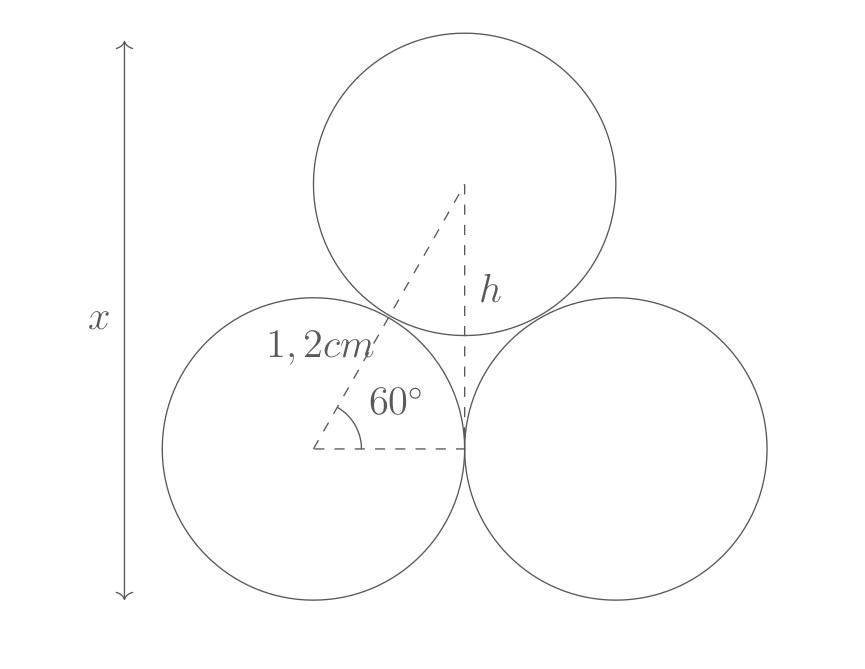
\includegraphics[width=\columnwidth,left]{../assets/geo.png}
        \end{column}
        \begin{column}{0.48\textwidth}
            \titlepage
        \end{column}
    \end{columns}

\end{frame}
}

%-------------------------------------------------------------------------------
% Sumário
%-------------------------------------------------------------------------------

\begin{frame}
    \frametitle{Sumário} % Table of contents slide, comment this block out to remove it
    \tableofcontents % Throughout your presentation, if you choose to use \section{} and \subsection{} commands, these will automatically be printed on this slide as an overview of your presentation
\end{frame}

%----------------------------------------------------------------------------------------
%	PRESENTATION SLIDES
%----------------------------------------------------------------------------------------

\section{Aulas anteriores}
\subsection{Revisão}
\begin{frame}[fragile]\frametitle{\subsecname}
    Até agora vimos como trabalhar com problemas que podem ser decompostos em um 
    ou mais triângulos retângulos, tanto através das funções trigonométricas e 
    suas relações com o triângulo retângulo, como também utilizando do Teorema 
    de Pitágoras, e por último vimos as Leis dos Cossenos que também nos auxiliam
    a trabalhar com problemas relacionados a triângulos.
\end{frame}

%------------------------------------------------

\begin{frame}\frametitle{\subsecname}
    \begin{block}{Relações trigonométricas}
        \begin{columns}
            \begin{column}{0.2\textwidth}
                \begin{align*}
                    sen(\theta) = \frac{CO}{hip}
                \end{align*}
            \end{column} 
            \begin{column}{0.2\textwidth}
                \begin{align*}
                    cos(\theta) = \frac{CA}{hip}
                \end{align*}
            \end{column} 
            \begin{column}{0.2\textwidth}
                \begin{align*}
                    tg(\theta) = \frac{CO}{CA}
                \end{align*}
            \end{column} 

        \end{columns}
    \end{block}

    \begin{block}{Teorema de Pitágoras}
        \begin{align*}
            a^2 = b^2 + c^2
        \end{align*}
    \end{block}

    \begin{block}{Lei dos Cossenos}
        \begin{align*}
            a^2 = b^2 + c^2 - 2\cdot b\cdot c\cdot cos(\alpha)\\
            b^2 = a^2 + c^2 - 2\cdot a\cdot c\cdot cos(\beta)\\ 
            c^2 = a^2 + b^2 - 2\cdot a\cdot b\cdot cos(\gamma)   
        \end{align*}
    \end{block}


\end{frame}


%------------------------------------------------

\section{Lei dos Senos}
% \subsection{Introdução}

\begin{frame}[fragile]\frametitle{\secname}
    Assim como a lei dos Cossenos, a lei dos Senos assemelha os comprimentos
    dos lados de um triângulo, dessa vez utilizando da função trigonométrica seno.
    \begin{figure}[H]
        \centering
        %\resizebox{\columnwidth}{!}{%
        \begin{tikzpicture}[scale=0.8\columnwidth/10cm]
            \coordinate (A) at (0,0);
            \coordinate (B) at (3,3);
            \coordinate (C) at (7,0);

            \draw (B)-- (C)-- (A)-- (B);
            \draw (A)-- node[above left] {$a$} (B); 
            \draw (B)-- node[right] {$c$} (C); 
            \draw (C)-- node[below] {$b$} (A); 
            \pic ["$\beta$", draw, -, angle eccentricity=2] {angle = A--B--C};
            \pic ["$\alpha$", draw, -, angle eccentricity=2] {angle = B--C--A};
            \pic ["$\gamma$", draw, -, angle eccentricity=2] {angle = C--A--B};
            
        \end{tikzpicture}
        %}
        % \caption{Triângulo retângulo $ABC$}
    \end{figure}

\end{frame}

%------------------------------------------------

\begin{frame}[fragile]\frametitle{\secname}
    \begin{figure}[H]
        \centering
        %\resizebox{\columnwidth}{!}{%
        \begin{tikzpicture}[scale=0.6\columnwidth/10cm]
            \coordinate (A) at (0,0);
            \coordinate (B) at (5,3);
            \coordinate (C) at (7,0);
            
            \draw (B)-- (C)-- (A)-- (B);
            \draw (A)-- node[above left] {$a$} (B); 
            \draw (B)-- node[right] {$c$} (C); 
            \draw (C)-- node[below] {$b$} (A); 
            \pic ["$\beta$", draw, -, angle eccentricity=2] {angle = A--B--C};
            \pic ["$\alpha$", draw, -, angle eccentricity=2] {angle = B--C--A};
            \pic ["$\gamma$", draw, -, angle eccentricity=2] {angle = C--A--B};
            
        \end{tikzpicture}
        %}
        % \caption{Triângulo retângulo $ABC$}
    \end{figure}
    % A Lei dos Cossenos é composta por 3 equações, sendo elas:
    % \begin{align*}
    %     a^2 = b^2 + c^2 - 2\cdot b\cdot c\cdot cos(\alpha)\\
    %     b^2 = a^2 + c^2 - 2\cdot a\cdot c\cdot cos(\beta)\\ 
    %     c^2 = a^2 + b^2 - 2\cdot a\cdot b\cdot cos(\gamma)   
    % \end{align*}
    \pause
    \begin{block}{A Lei dos Senos é composta por 3 igualdades:}
        \begin{align*}
            \frac{a}{sen(\alpha)} = \frac{b}{sen(\beta)} = \frac{c}{sen(\gamma)}
        \end{align*}
    \end{block}
    
\end{frame}

%------------------------------------------------

\begin{frame}\frametitle{\secname}
    Podemos decompor em 3 equações distintas:
    \begin{block}{}%{A Lei dos Senos é composta por 3 igualdades:}
        \begin{align*}
            \frac{a}{sen(\alpha)} = \frac{b}{sen(\beta)}
        \end{align*}
        \begin{align*}
            \frac{a}{sen(\alpha)} = \frac{c}{sen(\gamma)}
        \end{align*}
        \begin{align*}
            \frac{b}{sen(\beta)} = \frac{c}{sen(\gamma)}
        \end{align*}
    \end{block}
\end{frame}

%------------------------------------------------

\begin{frame}\frametitle{\secname}
    Note que podemos inverter as equações, tendo então
    \begin{block}{}%{A Lei dos Senos é composta por 3 igualdades:}
        \begin{align*}
            \frac{a}{sen(\alpha)} = \frac{b}{sen(\beta)} \rightarrow \frac{sen(\alpha)}{a} = \frac{sen(\beta)}{b}
        \end{align*}
        \begin{align*}
            \frac{a}{sen(\alpha)} = \frac{c}{sen(\gamma)} \rightarrow \frac{sen(\alpha)}{a} = \frac{sen(\gamma)}{c}
        \end{align*}
        \begin{align*}
            \frac{b}{sen(\beta)} = \frac{c}{sen(\gamma)} \rightarrow \frac{sen(\beta)}{b} = \frac{sen(\gamma)}{c}
        \end{align*}
    \end{block}
\end{frame}

%------------------------------------------------
\begin{frame}\frametitle{\secname}
    Portanto temos duas representações igualmente válidas para a Lei dos Senos:
    \begin{block}{}
        \begin{align*}
            \frac{a}{sen(\alpha)} = \frac{b}{sen(\beta)} = \frac{c}{sen(\gamma)}
        \end{align*}
    \end{block}
    e
    \begin{block}{}
        \begin{align*}
            \frac{sen(\alpha)}{a} = \frac{sen(\beta)}{b} = \frac{sen(\gamma)}{c}
        \end{align*}
    \end{block}
\end{frame}

%------------------------------------------------

%------------------------------------------------

\section{Exemplos}
\begin{frame}[fragile]\frametitle{\secname}
    \begin{block}{Exemplo 1.}
        Dado o triângulo abaixo, calcule o comprimento de $x$:
        \begin{figure}[H]
            \centering
            %\resizebox{\columnwidth}{!}{%
            \begin{tikzpicture}[scale=0.5\columnwidth/10cm]
                \coordinate (A) at (0,0);
                \coordinate (B) at (4,4);
                \coordinate (C) at (5,0);
                
                \draw (B)-- (C)-- (A)-- (B);
                \draw (A)-- (B); 
                \draw (B)-- node[above right] {$3cm$} (C); 
                \draw (C)-- node[below] {$x$} (A); 
                \pic ["$60^\circ$", draw, -, angle eccentricity=1.5] {angle = A--B--C};
                \pic ["$45^\circ$", draw, -, angle eccentricity=2] {angle = C--A--B};

            \end{tikzpicture}
            %}
            % \caption{Triângulo retângulo $ABC$}
        \end{figure}
    \end{block}

\end{frame}
%------------------------------------------------

\begin{frame}[fragile]\frametitle{\secname}
    \begin{columns}
        \begin{column}{0.5\columnwidth}
            \begin{figure}[H]
                % \centering
                %\resizebox{\columnwidth}{!}{%
                \begin{tikzpicture}[scale=1\columnwidth/10cm]
                    \coordinate (A) at (0,0);
                    \coordinate (B) at (4,4);
                    \coordinate (C) at (5,0);
                    
                    \draw (B)-- (C)-- (A)-- (B);
                    \draw (A)-- (B); 
                    \draw (B)-- node[above right] {$3cm$} (C); 
                    \draw (C)-- node[below] {$x$} (A); 
                    \pic ["$60^\circ$", draw, -, angle eccentricity=1.5] {angle = A--B--C};
                    \pic ["$45^\circ$", draw, -, angle eccentricity=2] {angle = C--A--B};
    
                \end{tikzpicture}
                %}
                % \caption{Triângulo retângulo $ABC$}
            \end{figure}
        \end{column}

        \begin{column}{0.5\textwidth}
            Vamos começar por escrever a equação que rege esse problema.
            \begin{align*}
                &\frac{x}{sen(60^\circ)} \pause = \frac{3}{sen(45^\circ)}\\
                \pause &x = \pause sen(60^\circ)\cdot\frac{3}{sen(45^\circ)}\\
                \pause &x = \pause \frac{\sqrt{3}}{2}\cdot\frac{3}{\frac{\sqrt{2}}{2}}\\
                \pause &x = \pause \frac{\sqrt{3}}{\cancel{2}}\cdot\frac{\cancel{2}}{\sqrt{2}}\cdot 3\\
                \pause &x = \pause 3\cdot\frac{\sqrt{3}}{\sqrt{2}} = \frac{3}{2}\sqrt{6}
            \end{align*}
        \end{column}
    \end{columns}

\end{frame}

%------------------------------------------------

% \section{Exemplos}
\begin{frame}[fragile]\frametitle{\secname}
    \begin{block}{Exemplo 2.}
        Dado o triângulo abaixo, calcule o comprimento de $x$:
        \begin{figure}[H]
            \centering
            %\resizebox{\columnwidth}{!}{%
            \begin{tikzpicture}[scale=0.5\columnwidth/10cm]
                \coordinate (A) at (1,0);
                \coordinate (B) at (3,4);
                \coordinate (C) at (7,0);
                
                \draw (B)-- (C)-- (A)-- (B);
                \draw (A)-- node[left] {$x$} (B); 
                \draw (B)-- node[above right] {$7cm$} (C); 
                \draw (C)--  (A); 
                \pic ["$60^\circ$", draw, -, angle eccentricity=2] {angle = C--A--B};
                \pic ["$30^\circ$", draw, -, angle eccentricity=1.5] {angle = B--C--A};
                
            \end{tikzpicture}
            %}
            % \caption{Triângulo retângulo $ABC$}
        \end{figure}
    \end{block}

\end{frame}

%------------------------------------------------

\section{Próximas aulas}
\begin{frame}[fragile]\frametitle{\secname}
    \textbf{(Se folgarmos nos feriados)}
    \begin{itemize}
        \item \textcolor{red}{12/10 - Feriado (Nossa Senhora Aparecida)}
        \item 19/10 - Resolução de exercícios de vestibular
        \item 26/10 - Revisão de álgebra I
        \item \textcolor{red}{02/11 - Feriado (Finados)}
        \item 09/11 - Revisão de álgebra II 
        \item 16/11 - Volume, área e perímetro
        \item 23/11 - Aula de dúvidas
    \end{itemize}

\end{frame}

%------------------------------------------------

% \section{Próximas aulas}
\begin{frame}[fragile]\frametitle{\secname}
    \textbf{(Se não folgarmos nos feriados)}
    \begin{itemize}
        \item 12/10 - Resolução de exercícios de vestibular
        \item 19/10 - Revisão de álgebra I
        \item 26/10 - Revisão de álgebra II
        \item 02/11 - Volume, área e perímetro
        \item 09/11 - Volume, área e perímetro II 
        \item 16/11 - Resolução de exercícios de vestibular
        \item 23/11 - Aula de dúvidas
    \end{itemize}

\end{frame}

%------------------------------------------------


\begin{frame}
    \Huge{\centerline{Perguntas?}}
\end{frame}

%----------------------------------------------------------------------------------------

\end{document}